\subsection{Pole placement}\label{chapter_PolePlacementIMPL}

There are two requirements, that have to be checked before starting with the pole placement. First one is, that the physical process, that shall be controlled, is available as a linear mathematical model - e.g in Simulink. The other one is, that this process is controllable. Chapter \ref{chapter_StateSpaceIMPL} deals with that fact. 

First of all it is necessary to check where the poles of the process are. This can be done with the following MATLAB code.

\begin{lstlisting}
	System = linmod('dynamics_reduced_without_motordelay');
	StateSpace = ss(System.a, System.b, System.c, System.d);
	eig(StateSpace) 
	pzmap(StateSpace)        
\end{lstlisting}

The output of the eig() function is:
\begin{lstlisting}
         0
    0.2378
   -0.2378
         0
         0       
\end{lstlisting}

And the pole/zero-map looks like that:
\begin{figure}
	\centering
		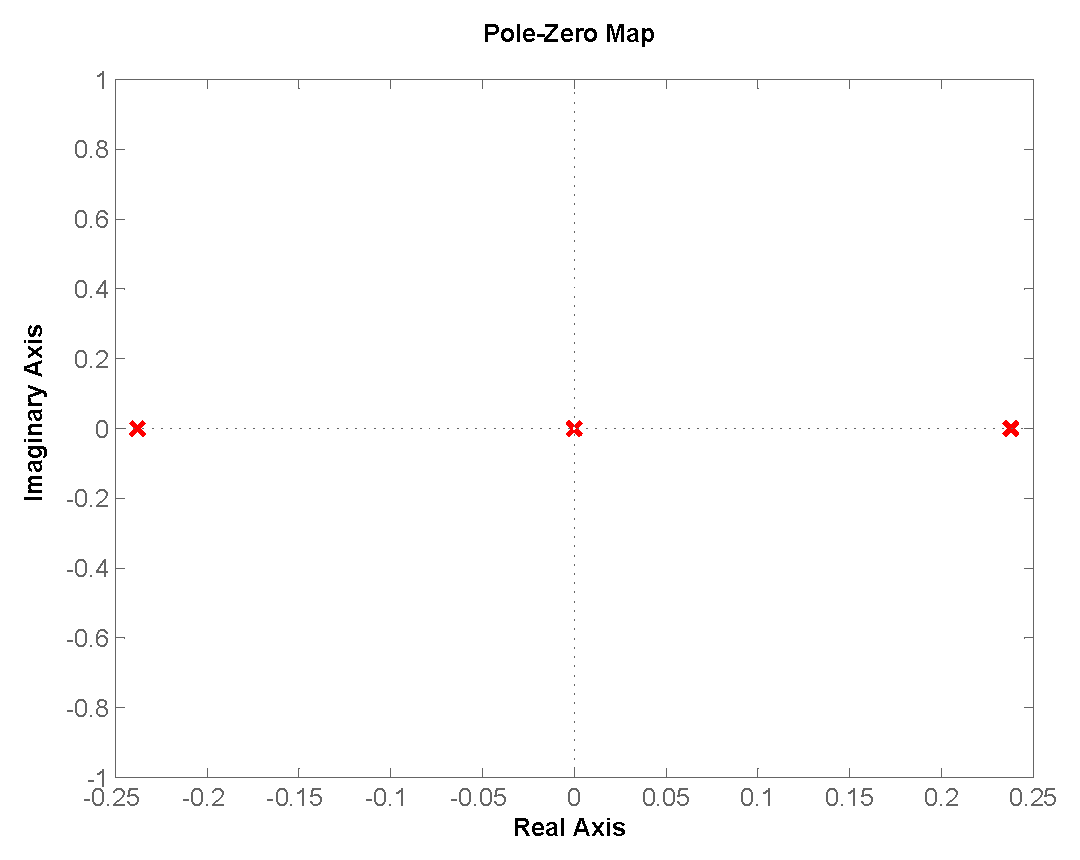
\includegraphics[width=0.70\textwidth]{03_Grafiken/PZmap_process.pdf}
	\caption{Pole/zero-map of the reduced quadrocopter process}
	\label{fig:PZmap_process}
\end{figure}


So there are five poles - three at zero, one at 0.2378 and one at -0.2378. This pole constellation - and consequently the process - is not stable, because one pole is at the right half-plane. So it is coercible necessary to use a controller for that process. The function of the pole placement is, to move at least the positive pole to the left half-plane. The three poles at zero are also not really nice, because they are not stable like the pole on the left half-plane. Poles on the imaginary axis can oscillate without damping. So the first requirement is, that all poles have to be moved to the left half-plane.
Next step is thinking about, to which values the poles should be moved. For an aircraft overshooting is not a good feature. So the second requirement is, that all poles have to stay at the real axis of the s-plane. And the third requirement is, that the poles, corresponding to the rates, have to be faster than those, belonging to the angles. 

To challenge all these requirements, the poles are moved to [-18 -5 -7 -10 -9]. Maybe these poles are too fast and they have to be moved to lower negative values. But it is not possible to know about that at this step of the development. Chapter \ref{chapter_TEST} deals with that circumstance.